% ------------------------------------------------------------------------------
% TYPO3 CMS 7.4 - What's New - Chapter "Introduction" (English Version)
%
% @author	Michael Schams <schams.net>
% @license	Creative Commons BY-NC-SA 3.0
% @link		http://typo3.org/download/release-notes/whats-new/
% @language	English
% ------------------------------------------------------------------------------
% LTXE-CHAPTER-UID:		9dc37b9a-9fad14c3-bf7eabfd-82b83622
% LTXE-CHAPTER-NAME:	Introduction
% ------------------------------------------------------------------------------

\section{Uvod}
\begin{frame}[fragile]
	\frametitle{Uvod}

	\begin{center}\huge{Uvod}\end{center}
	\begin{center}\huge{\color{typo3darkgrey}\textbf{Cinjenice}}\end{center}

\end{frame}

% ------------------------------------------------------------------------------
% LTXE-SLIDE-START
% LTXE-SLIDE-UID:		3dbd13c5-d23b5dd4-0060851b-ba7a5b4d
% LTXE-SLIDE-ORIGIN:	3cc566cf-d7166203-45a36415-7c8e8ebf English
% LTXE-SLIDE-ORIGIN:	5d8622ac-37911548-171bf8ec-5add4ed5 German
% LTXE-SLIDE-TITLE:		TYPO3 CMS 7.4 - The Facts
% ------------------------------------------------------------------------------
\begin{frame}[fragile]
	\frametitle{Uvod}
	\framesubtitle{TYPO3 CMS 7.4 - Cinjenice}

	\begin{itemize}
		\item Datum objavljivanja: 04. Avgust 2015
		\item Tip objavljivanja: "Brza objava" ("Sprint Release")
		\item Vizija: Prihvatiti, inovirati, dostaviti
		\item Glavni fokus: Remont administratorskog interfejsa drugi deo
	\end{itemize}

\end{frame}

% ------------------------------------------------------------------------------
% LTXE-SLIDE-START
% LTXE-SLIDE-UID:		454f3ece-0a54b367-ed499f7c-9fa1cdf6
% LTXE-SLIDE-ORIGIN:	6746e3bc-a8575d0c-e1681766-d0d78911 English
% LTXE-SLIDE-ORIGIN:	9da27f39-55d99c31-9ee9136a-20d96c0e German
% LTXE-SLIDE-TITLE:		System Requirements
% ------------------------------------------------------------------------------
\begin{frame}[fragile]
	\frametitle{Uvod}
	\framesubtitle{Sistemski zahtevi}

	\begin{itemize}
		\item PHP*:\tabto{3cm}v5.5.0 - v5.6.x
		\item MySQL:\tabto{3cm}v5.5.x - v5.6.x (no strict mode)
		\item Prostor na disku:\tabto{3cm}min 200 MB
		\item PHP podesavanja:

			\begin{itemize}
				\item memory\_limit >= 128M
				\item max\_execution\_time >= 240s
				\item opcija \texttt{--disable-ipv6} \underline{ne sme} se koristit
			\end{itemize}

		\item Administratorski interfejs zahteva IE >= 9 ili bilo koji drugi moderni pretrazivac

	\end{itemize}

	\vspace{1cm}
	*) Dodatno objasnjenje: \href{http://typo3.org/news/article/php-minimum-requirements-for-typo3-cms-7/}{PHP Minimum Requirements for TYPO3 CMS 7}

\end{frame}

% ------------------------------------------------------------------------------
% LTXE-SLIDE-START
% LTXE-SLIDE-UID:		0722e90a-f22d4723-f220b808-da3cde6b
% LTXE-SLIDE-ORIGIN:	081f8b1d-b8f58841-dccf8d1d-148fd25d English
% LTXE-SLIDE-ORIGIN:	dbbfebbe-fb43ddb8-bca9ae69-716b8a0f German
% LTXE-SLIDE-TITLE:		Development And Release Timeline
% ------------------------------------------------------------------------------
\begin{frame}[fragile]
	\frametitle{Uvod}
	\framesubtitle{Vreme razvoja i datumi objavljivanja}

	\begin{figure}
		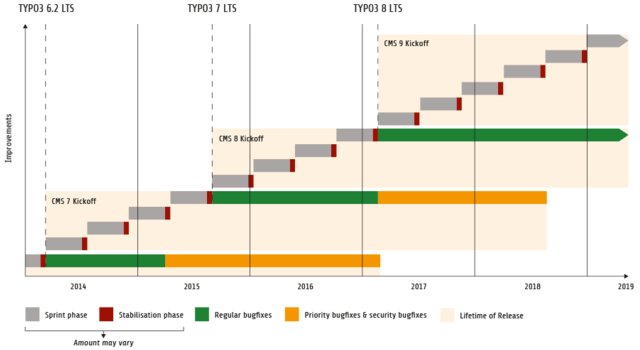
\includegraphics[width=0.90\linewidth]{Introduction/ReleaseAgenda.png}
	\end{figure}

\end{frame}

% ------------------------------------------------------------------------------
% LTXE-SLIDE-START
% LTXE-SLIDE-UID:		4162ec26-6a57b2c5-9debb376-8b346cc1
% LTXE-SLIDE-ORIGIN:	a5555bb0-f1f8031f-f271766a-2dbc1b08 English
% LTXE-SLIDE-ORIGIN:	e359142e-e7c10774-5d851da9-b26a275b German
% LTXE-SLIDE-TITLE:		TYPO3 CMS Roadmap
% ------------------------------------------------------------------------------
\begin{frame}[fragile]
	\frametitle{Uvod}
	\framesubtitle{TYPO3 CMS plan}

	Predvidjeni datumi objavljivanja i njihov osnovni fokus:

	\begin{itemize}
		\item v7.0 \tabto{1.0cm}02/Dec/2014\tabto{3.4cm}Remont administratorskog interfejsa prvi deo
		\item v7.1 \tabto{1.0cm}24/Feb/2015\tabto{3.4cm}Ciscenje osnove sistema i optimizacija
		\item v7.2 \tabto{1.0cm}28/Apr/2015\tabto{3.4cm}Korisnicki interfejs
		\item v7.3 \tabto{1.0cm}16/Jun/2015\tabto{3.4cm} Ekosistem za dodatke, Composer\newline
			\tabto{3.4cm} i upravljanje prosirenjima
		\item
			\begingroup
				\color{typo3orange}
					v7.4 \tabto{1.0cm}04/Aug/2015\tabto{3.4cm}Remont administratorskog interfejsa drugi deo
			\endgroup

		\item v7.5 \tabto{1.0cm}29/Sep/2015\tabto{3.4cm}\textit{(bice odredjeno...)}
		\item v7.6 \tabto{1.0cm}xx/xxx/2015\tabto{3.4cm}\textbf{TYPO3 CMS 7 LTS}\newline
			\tabto{3.4cm}(Verzija sa dugorocnom podrskom)
	\end{itemize}

	\smaller
		\url{https://typo3.org/typo3-cms/roadmap/}\newline
		\url{http://typo3.org/news/article/embrace-and-innovate-typo3-cms-7/}
	\normalsize

\end{frame}

% ------------------------------------------------------------------------------
% LTXE-SLIDE-START
% LTXE-SLIDE-UID:		d3515e43-427dbf84-c2d74160-783c47a1
% LTXE-SLIDE-ORIGIN:	5ef3ad6d-b72464d3-6a2867a6-298cb382 English
% LTXE-SLIDE-ORIGIN:	c8966352-3e5159b9-f0e3ea35-9d4455ef German
% LTXE-SLIDE-TITLE:		Installation
% ------------------------------------------------------------------------------
\begin{frame}[fragile]
	\frametitle{Uvod}
	\framesubtitle{Instalacija}

	\begin{itemize}
		\item Zvanicna procedura za instalaciju na Linux/Mac OS X\newline
			(DocumentRoot na primer \texttt{/var/www/site/htdocs}):
		\begin{lstlisting}
			$ cd /var/www/site
			$ wget --content-disposition get.typo3.org/7.4
			$ tar xzf typo3_src-7.4.0.tar.gz
			$ cd htdocs
			$ ln -s ../typo3_src-7.4.0 typo3_src
			$ ln -s typo3_src/index.php
			$ ln -s typo3_src/typo3
			$ touch FIRST_INSTALL
		\end{lstlisting}

		\item Simbolicki linkovi (Symbolic links) na Microsoft Windows:

			\begin{itemize}
				\item Koristiti \texttt{junction} za Windows XP/2000
				\item Koristiti \texttt{mlink} za Windows Vista i Windows 7
			\end{itemize}

	\end{itemize}
\end{frame}

% ------------------------------------------------------------------------------
% LTXE-SLIDE-START
% LTXE-SLIDE-UID:		dd915153-b727c58c-0b146ba8-abfe20cc
% LTXE-SLIDE-ORIGIN:	12551741-9cb07199-fb3614d0-1a242a5f English
% LTXE-SLIDE-ORIGIN:	af099855-2b970b2b-89ed7d02-7219b2b9 German
% LTXE-SLIDE-TITLE:		Upgrade to TYPO3 CMS 7
% ------------------------------------------------------------------------------
\begin{frame}[fragile]
	\frametitle{Uvod}
	\framesubtitle{Nadogradnja na TYPO3 CMS 7.x}

	\begin{itemize}
		\item Nadogradnja je moguca samo sa TYPO3 CMS 6.2 LTS
		\item TYPO3 CMS < 6.2 bi prvo trebalo nadograditi na TYPO3 CMS 6.2 LTS
	\end{itemize}

	\begin{itemize}

		\item Upsutstvo za nadogradnju:\newline
			\smaller\url{http://wiki.typo3.org/Upgrade#Upgrading_to_7.3}\normalsize
		\item Zvanicni TYPO3 vodic "TYPO3 Installation and Upgrading":
			\smaller\url{http://docs.typo3.org/typo3cms/InstallationGuide}\normalsize
		\item Opsti pristup:
			\begin{itemize}
				\item Proveriti minimalne sistemske zahte \small(PHP, MySQL, itd.)
				\item Proveriti \textbf{deprecation\_*.log} u staroj TYPO3 instanci
				\item Nadograditi sva prosirenja na najnoviju verziju
				\item Postaviti nove fajlove i pokrenuti Install Tool \textrightarrow Upgrade Wizard
				\item Proveriti startup modul za administratore (opciono)
			\end{itemize}
	\end{itemize}

\end{frame}

% ------------------------------------------------------------------------------
